% !TEX root = ../tex/5-4.tex
% 第5章：本文は青、補足は緑
\newcommand{\asmain}{%
    \setbeamercolor{frametitle}{fg=white,bg=main}%
    \setbeamercolor{structure}{fg=main}%
    \setbeamercolor{itemize item}{fg=main}%
    \setbeamercolor{itemize subitem}{fg=main}%
    \setbeamercolor{enumerate item}{fg=main}%
}
\newcommand{\assuppl}{%
    \setbeamercolor{frametitle}{fg=white,bg=examplecol}%
    \setbeamercolor{structure}{fg=examplecol}%
    \setbeamercolor{itemize item}{fg=examplecol}%
    \setbeamercolor{itemize subitem}{fg=examplecol}%
    \setbeamercolor{enumerate item}{fg=examplecol}%
}
% フレームタイトルの「補足」だけを□で囲む
\newcommand{\supplmark}{%
    \setlength{\fboxsep}{1.5pt}%
    \setlength{\fboxrule}{0.7pt}%
    \fbox{\textbf{補足}}%
}
\asmain


%=============================================
\begin{frame}{5.4 (Optional)：Canonical Affine Flow}
    \begin{block}{この節の位置づけ（論文 5.4）}
        線形（canonical affine）経路の性質と、\\
        周辺軌道を真っ直ぐに近づける Rectify / Reflow。
    \end{block}
    \begin{itemize}
        \item 独立カップリングでは条件付きは直線でも、周辺ODEは曲がりうる
        \item Rectify：学習した流れで端点を結び直す
        \item Reflow：それを反復し、少数ステップ積分を楽にする
    \end{itemize}
    \vfill
    \footnotesize
    任意節。初読は概要だけでも可。詳細は緑（補足）で。
\end{frame}
%=============================================
\asmain
\begin{frame}{5.4 の道筋（概要）}
    \begin{enumerate}
        \item \textbf{Canonical affine path}\\
        $x_t=(1-t)x_0+tx_1$。目的関数が $v_\phi\approx x_1-x_0$ に単純化
        \item \textbf{Rectify（5.4.1）}\\
        独立ペア $\to$ 学習ODEが誘導する従属カップリング
        \item \textbf{Reflow（5.4.2--5.4.3）}\\
        Rectifyの反復。輸送コスト非増加と直線化の性質
    \end{enumerate}
\end{frame}
%=============================================
\section{Canonical Affine Path}
\assuppl
\begin{frame}{\supplmark：線形補間経路}
    端点分布 $p_0=p_{\mathrm{src}}$、$p_1=p_{\mathrm{tgt}}$ に対し
    \[
        a_t=1-t,\qquad b_t=t,
        \qquad
        x_t=(1-t)x_0+tx_1
    \]
    （$x_0\sim p_{\mathrm{src}}$、$x_1\sim p_{\mathrm{tgt}}$）。
    学習目標は
    \[
        \mathbb{E}_{t,x_0,x_1}
        \bigl\|
            v_\phi(x_t,t)-(x_1-x_0)
        \bigr\|_2^{2}.
    \]
    \begin{exampleblock}{ねらい}
        この線形流は Reflow による反復的な直線化と相性が良い。
    \end{exampleblock}
\end{frame}
%=============================================
\section{5.4.1 Rectifying Flows}
\assuppl
\begin{frame}{\supplmark：なぜカップリングを変えるか}
    独立カップリング
    \[
        \pi(x_0,x_1)=p_{\mathrm{src}}(x_0)\,p_{\mathrm{tgt}}(x_1)
    \]
    では、各条件付き補間 $(1-t)x_0+tx_1$ は直線である。
    \begin{itemize}
        \item しかし周辺速度は無関係な端点ペアの方向を平均する
        \item 誘導される周辺ODE軌道は曲がりうる
        \item 少数の数値ステップでは積分誤差が増えやすい
    \end{itemize}
    \begin{alertblock}{Rectificationの発想}
        端点の結び方を、学習済み流れが作る従属カップリングに置き換える。
    \end{alertblock}
\end{frame}
%=============================================
\assuppl
\begin{frame}{\supplmark：Rectify操作（Algorithm 2）}
    事前学習した速度 $v_{\phi^\times}$ をドリフトとする PF-ODE
    \[
        \frac{\mathrm{d}z(t)}{\mathrm{d}t}
        = v_{\phi^\times}(z(t),t),
        \qquad
        z(0)=z_0\sim p_{\mathrm{src}}
    \]
    を $t\in[0,1]$ で積分し、$\hat{z}_1:=z(1)$ を得る。
    \begin{enumerate}
        \item \textbf{Pre-Train}：選んだ経路上で $v_\phi\approx \dot{x}_t$ を学習
        \item \textbf{Rectify}：$(z_0,\hat{z}_1)$ の従属ペアを出力
    \end{enumerate}
    \begin{exampleblock}{読み方}
        任意の独立ペアではなく、モデルが運んだ端点で次の補間を組む。
    \end{exampleblock}
\end{frame}
%=============================================
\assuppl
\begin{frame}{\supplmark：周辺を保つ構造}
    流マップを $\Phi_{0\to t}$ と書くと $z(t)=\Phi_{0\to t}(z_0)$、
    $\hat{z}_1=\Phi_{0\to 1}(z_0)$。
    \[
        \pi_{\mathrm{Rectify}}(z_0,z_1)
        =
        p_{\mathrm{src}}(z_0)\,
        \delta\!\bigl(z_1-\Phi_{0\to 1}(z_0)\bigr).
    \]
    \begin{itemize}
        \item \textbf{ソース周辺は不変：}
        $\int \pi_{\mathrm{Rectify}}(z_0,z_1)\,\mathrm{d}z_1=p_{\mathrm{src}}(z_0)$
        \item \textbf{押し出し：}
        $(\Phi_{0\to t})_{\#}p_{\mathrm{src}}=\mathrm{Law}(z(t))$
        \item 理想速度なら $\mathrm{Law}(z(t))=\mathrm{Law}(x_t)$、かつ
        $(\Phi_{0\to 1})_{\#}p_{\mathrm{src}}=p_{\mathrm{tgt}}$
    \end{itemize}
\end{frame}
%=============================================
\section{5.4.2 Reflow}
\assuppl
\begin{frame}{\supplmark：Question 5.4.1}
    \begin{block}{問い}
        正しい周辺を保ちつつ、\\
        より直線に近い輸送経路を誘導するカップリングを学べるか？
    \end{block}
    \begin{itemize}
        \item 独立ペアは曲がりくねった周辺軌道を招きやすい
        \item 離散化誤差とシミュレーション分散が増える
        \item \textbf{Reflow}：Rectify を繰り返し、カップリングを更新する
    \end{itemize}
\end{frame}
%=============================================
\assuppl
\begin{frame}{\supplmark：Reflowの1反復}
    現在のカップリング $\pi^{(k)}$ に対し、
    \begin{enumerate}
        \item \textbf{再学習}
        \[
            \mathcal{L}\!\bigl(\phi;\pi^{(k)}\bigr)
            =
            \mathbb{E}_{t,(z_0,\hat{z}_1)\sim\pi^{(k)}}
            \bigl\|
                v_\phi(z_t,t)-(\hat{z}_1-z_0)
            \bigr\|_2^{2}
            \tag{5.4.1}
        \]
        （$z_t=(1-t)z_0+t\hat{z}_1$）
        \item \textbf{新カップリング}
        新しい $z_0\sim p_{\mathrm{src}}$ から学習ODEを積分し $\hat{z}_1$ を得る
    \end{enumerate}
    \[
        \pi^{(k+1)}=\mathrm{Rectify}\!\bigl(\pi^{(k)}\bigr)
        \tag{5.4.2}
    \]
\end{frame}
%=============================================
\section{5.4.3 Properties of Reflow}
\assuppl
\begin{frame}{\supplmark：性質 I：輸送コストは増えない}
    凸コスト $c$（例：$\|y\|_2^p$、$p\ge 1$）に対し、
    \begin{block}{Proposition 5.4.1}
        理想速度 $v^*=v_{\phi^\times}$ の下で
        \[
            \mathbb{E}\bigl[c(\hat{z}_1-z_0)\bigr]
            \le
            \mathbb{E}\bigl[c(x_1-x_0)\bigr].
        \]
    \end{block}
    \begin{itemize}
        \item Jensen 不等式に由来（詳細は Liu, Gong et al., 2022）
        \item 再帰適用より、Reflow 列は輸送コストを増やさない
    \end{itemize}
\end{frame}
%=============================================
\assuppl
\begin{frame}{\supplmark：性質 II：経路の直線化}
    経路 $Y=\{y_t\}$ の直線性汎関数
    \[
        S(Y)
        :=
        \int_0^1
        \mathbb{E}
        \Bigl\|
            y_1-y_0-\frac{\mathrm{d}y_t}{\mathrm{d}t}
        \Bigr\|_2^{2}
        \,\mathrm{d}t.
    \]
    $S(Y)=0$ なら完全な直線。
    \begin{block}{Proposition 5.4.2}
        整流された経路 $Z^{(k)}$ について
        \[
            \min_{k\in\{0,\ldots,K\}}
            S(Z^{(k)})
            \le
            \frac{\mathbb{E}\|x_1-x_0\|_2^{2}}{K}.
        \]
    \end{block}
    \footnotesize
    各反復で単調改善するとは限らないが、$K$ 回のうち最良は $O(1/K)$ で良い。
\end{frame}
%=============================================
\assuppl
\begin{frame}{\supplmark：Figure 5.11 --- Reflowの直感}
    \centering
    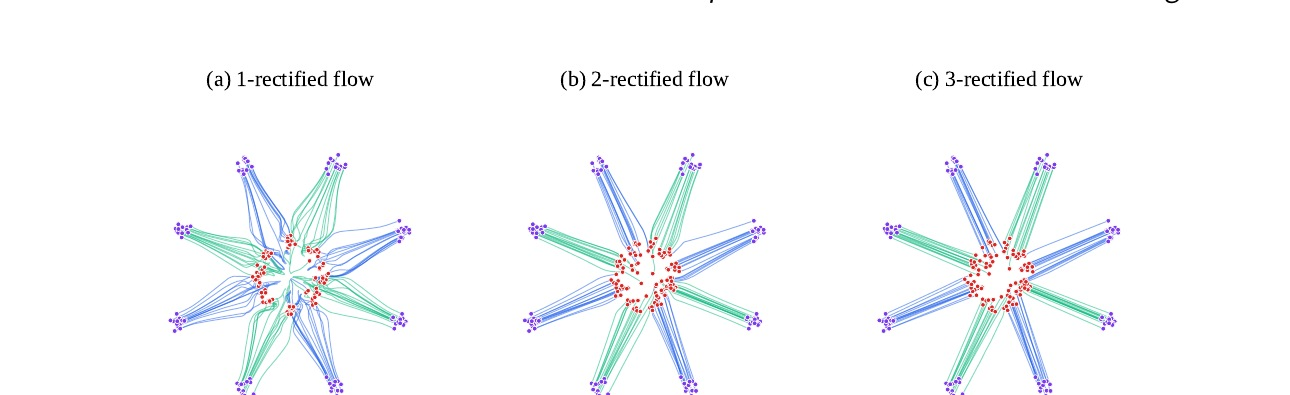
\includegraphics[width=0.95\textwidth]{fig-5-11.jpg}
    \vfill
    \footnotesize
    反復ごとに周辺軌道が真っ直ぐに近づく（1 / 2 / 3-rectified）。\\
    Source: Adapted from Liu, Gong, et al.\ (2022).
\end{frame}
%=============================================
\assuppl
\begin{frame}{\supplmark：OTとの関係（予告）}
    直線カップリングは二次コスト OT の\textbf{必要条件}だが、\\
    \textbf{十分条件ではない}。
    \begin{itemize}
        \item OTマップ $T$ では $x_t=(1-t)x_0+tT(x_0)$ が直線
        \item 任意の $S$ による直線 $x_t=(1-t)x_0+tS(x_0)$ が最適とは限らない
        \item 最適性は Monge コスト $\mathbb{E}\|x_0-S(x_0)\|_2^{2}$ の最小化にも依存
    \end{itemize}
    \begin{exampleblock}{先送り}
        用語と詳細は 7.2 / 7.5.2。ここでは「真っ直ぐ $\neq$ OT最適」と覚える。
    \end{exampleblock}
\end{frame}
%=============================================
\asmain
\begin{frame}{5.4 のまとめ（任意節）}
    \begin{itemize}
        \item Canonical affine：$x_t=(1-t)x_0+tx_1$、目標は $x_1-x_0$
        \item Rectify：独立ペアを、学習流れの従属カップリングへ置き換える
        \item Reflow：Rectifyの反復。コスト非増加＋直線化の保証
        \item 少数ステップ積分を楽にする実用的な整流手続き
        \item 直線化は OT 最適の必要だが十分ではない（詳細は第7章）
    \end{itemize}
    \begin{block}{本編との関係}
        5.2--5.3 の FM 本体の上に乗る「経路を綺麗にする」道具箱。
    \end{block}
\end{frame}
%=============================================
\asmain
\begin{frame}{次節へ：Closing Remarks}
    任意の整流の話を終え、第5章全体を閉じる。
    \begin{enumerate}
        \item NF $\to$ NODE $\to$ Flow Matching の道筋を振り返る
        \item Score SDE との対応（同じ確率流・学ぶ量が違う）
        \item 到達目標のチェックと、第6章の統一レンズへ
    \end{enumerate}
\end{frame}
